\section{Laplace变换求解}
\label{sec:lde-laplace}

常系数方程的公式已经齐备，但计算$\mathrm{e}^{t\bm{A}}$和卷积积分有时并不轻松。另一条路线是把求导变成乘法，把初值自动放进代数方程，再把结果翻译回时间域。这条路线要回答三件事：变换何时有定义，初值怎样进入，反过来的翻译是否唯一？

\paragraph{用指数权给函数“称重”}
考虑积分$\int_0^{\infty}\mathrm{e}^{-zt}f(t)\,\mathrm{d}t$。$\mathrm{e}^{-zt}$是一个衰减的权，$z$的实部越大，权衰减得越快，增长的函数也能被压住。图~\ref{fig:lde-laplace-weight}取$f=\mathrm{e}^{t}$：$z=0.5$时乘积仍在增长，$z=1$时是常数，只有$z=2$时乘积衰减，积分收敛。

把$z$取遍一个半平面，就得到一族读数，它们记录了$f$的全部信息。与Fourier变换相比，这里只积分$t\geq0$，并带有衰减权，所以允许指数增长的函数；当$z$在虚轴上时，它就是$f\mathbb{I}_{[0,\infty)}$的Fourier变换。后者的性质可参考\BookChapterRef{chap:fourier-transform}{卷四第14章“Fourier变换”}。

\begin{BookInlineFigure}
  \centering
  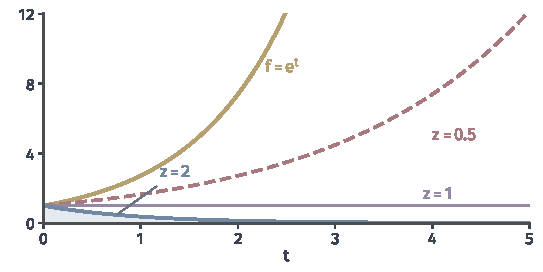
\includegraphics[width=92mm]{figures/06-differential-equations/01-ordinary-differential-equations/matplotlib/lde-laplace-weight/figure.pdf}
  \caption{指数权压住增长。黄线是$f=\mathrm{e}^{t}$，其余曲线是乘积$\mathrm{e}^{-zt}f(t)$：红色虚线$z=0.5$仍增长，紫线$z=1$恒为$1$，蓝线$z=2$衰减，浅蓝是收敛积分的面积$1$。}
  \label{fig:lde-laplace-weight}
\end{BookInlineFigure}

\begin{definition}[单边Laplace变换]
\label{def:lde-laplace}
设$f:[0,\infty)\to\mathbb{C}$在每个有界区间上分段连续（有限个间断点，左右极限都有限），且存在常数$M\geq0$和$c\in\mathbb{R}$使$\lvert f(t)\rvert\leq M\mathrm{e}^{ct}$对所有$t\geq0$成立，就称$f$是\term{指数阶函数}（function of exponential order）。对$\operatorname{Re}z>c$，定义$f$的\term{单边Laplace变换}（unilateral Laplace transform）
\begin{equation}
 \hat{f}(z)=\mathcal{L}[f](z)=\int_0^{\infty}\mathrm{e}^{-zt}f(t)\,\mathrm{d}t.
 \label{eq:lde-laplace}
\end{equation}
\end{definition}

记$\sigma=\operatorname{Re}z$。$\sigma>c$时被积函数的模不超过$M\mathrm{e}^{-(\sigma-c)t}$，所以积分绝对收敛，并且$\lvert\hat{f}(z)\rvert\leq M/(\sigma-c)$。不是每个函数都有变换：$\mathrm{e}^{t^2}$增长得比任何指数都快，对任何$z$积分都发散。

\paragraph{常用变换对}
直接积分可得$\mathcal{L}[\mathrm{e}^{at}](z)=1/(z-a)$，收敛条件是$\operatorname{Re}z>\operatorname{Re}a$。令$a$取$\pm\mathrm{i}\beta$再线性组合，得到正弦和余弦；对$a$逐次求导，得到$t^k\mathrm{e}^{at}$。表~\ref{tab:lde-laplace-pairs}列出本节用到的结果。

\begin{BookInlineTable}
  \centering
  \caption{常用的单边Laplace变换对，$k$为非负整数，$a\in\mathbb{C}$，$\beta,\tau$为实数，$\tau\geq0$。}
  \label{tab:lde-laplace-pairs}
  \begin{tabular}{lll}
    \toprule
    $f(t)$ & $\hat{f}(z)$ & 收敛范围\\
    \midrule
    $\mathrm{e}^{at}$ & $1/(z-a)$ & $\operatorname{Re}z>\operatorname{Re}a$\\
    $t^k\mathrm{e}^{at}$ & $k!/(z-a)^{k+1}$ & $\operatorname{Re}z>\operatorname{Re}a$\\
    $\cos\beta t$ & $z/(z^2+\beta^2)$ & $\operatorname{Re}z>0$\\
    $\sin\beta t$ & $\beta/(z^2+\beta^2)$ & $\operatorname{Re}z>0$\\
    $\mathrm{e}^{at}f(t)$ & $\hat{f}(z-a)$ & $\operatorname{Re}z>c+\operatorname{Re}a$\\
    $f(t-\tau)\mathbb{I}_{[\tau,\infty)}(t)$ & $\mathrm{e}^{-\tau z}\hat{f}(z)$ & $\operatorname{Re}z>c$\\
    \bottomrule
  \end{tabular}
\end{BookInlineTable}

\paragraph{导数公式：初值从这里进入}
方程能被化成代数式，靠的是下面的公式。它也说明了连续性为什么不能省略。

\begin{theorem}[导数的Laplace变换]
\label{thm:lde-laplace-derivative}
设$f$在$[0,\infty)$上连续，分段连续可微，$\dot{f}$是指数阶函数，$\lvert\dot{f}(t)\rvert\leq M\mathrm{e}^{ct}$，其中$c>0$。则$f$也是指数阶函数，并且对$\operatorname{Re}z>c$，
\begin{equation}
 \mathcal{L}[\dot{f}](z)=z\hat{f}(z)-f(0).
 \label{eq:lde-laplace-derivative}
\end{equation}
\end{theorem}

\begin{proof}
由$f(t)=f(0)+\int_0^t\dot{f}$，得到
\[
 \lvert f(t)\rvert\leq\lvert f(0)\rvert+\frac{M}{c}\mathrm{e}^{ct},
\]
所以$f$是指数阶函数。

设$\dot{f}$的间断点为$t_1<t_2<\cdots$。在每一段上分部积分，并把$[0,T]$上的各段相加。$f$连续，所以内部接缝处的边界项两两抵消，只剩两端：
\[
 \int_0^T\mathrm{e}^{-zt}\dot{f}(t)\,\mathrm{d}t=\mathrm{e}^{-zT}f(T)-f(0)+z\int_0^T\mathrm{e}^{-zt}f(t)\,\mathrm{d}t.
\]
$\operatorname{Re}z>c$时，$\lvert\mathrm{e}^{-zT}f(T)\rvert\to0$。令$T\to\infty$就得到结论。
\end{proof}

连续性用在边界项的抵消上。若$f$有跳变，比如$f=\mathbb{I}_{[1,\infty)}$，则$\dot{f}$几乎处处为零，$\mathcal{L}[\dot{f}]=0$；而$z\hat{f}(z)-f(0)=\mathrm{e}^{-z}\neq0$，差额恰好是跳变项。

把公式用两次，得到二阶导数的变换：
\begin{equation}
 \mathcal{L}[\ddot{f}](z)=z^2\hat{f}(z)-zf(0)-\dot{f}(0).
 \label{eq:lde-laplace-second}
\end{equation}
这里要求$f$和$\dot{f}$连续。初值以多项式的形式出现在右端，所以不需要先求通解、再定常数。

\paragraph{卷积与唯一性}
式~\eqref{eq:lde-convolution-response}的卷积也有简单的像。对$[0,\infty)$上的函数，记$(f*g)(t)=\int_0^tf(t-s)g(s)\,\mathrm{d}s$。

\begin{theorem}[卷积定理]
\label{thm:lde-laplace-convolution}
设$f,g$是指数阶函数，相应的增长指数都不超过$c$。则$f*g$连续并且是指数阶函数，对$\operatorname{Re}z>c$有
\begin{equation}
 \mathcal{L}[f*g](z)=\hat{f}(z)\hat{g}(z).
 \label{eq:lde-laplace-convolution}
\end{equation}
\end{theorem}

\begin{proof}
由$\lvert f\rvert\leq M_1\mathrm{e}^{ct}$和$\lvert g\rvert\leq M_2\mathrm{e}^{ct}$，得$\lvert(f*g)(t)\rvert\leq M_1M_2t\mathrm{e}^{ct}$，它不超过常数乘$\mathrm{e}^{c't}$（任取$c'>c$）。连续性可由控制收敛定理得到。

设$\sigma=\operatorname{Re}z>c$。二重积分
\[
 \int_0^{\infty}\!\!\int_0^t\lvert\mathrm{e}^{-zt}f(t-s)g(s)\rvert\,\mathrm{d}s\,\mathrm{d}t\leq\frac{M_1M_2}{(\sigma-c)^2}
\]
有限：非负被积函数可以先对$t$积分，令$r=t-s$就得到右端的界。所以可用Fubini定理交换积分次序，同样令$r=t-s$：
\[
 \int_0^{\infty}\!\!\int_s^{\infty}\mathrm{e}^{-zt}f(t-s)g(s)\,\mathrm{d}t\,\mathrm{d}s=\int_0^{\infty}\mathrm{e}^{-zs}g(s)\,\mathrm{d}s\int_0^{\infty}\mathrm{e}^{-zr}f(r)\,\mathrm{d}r.
\]
右端正是$\hat{f}(z)\hat{g}(z)$。
\end{proof}

从像函数翻译回时间函数，要先知道翻译是唯一的。函数在个别点上的取值不影响积分，所以唯一性只能精确到这些点。

\begin{theorem}[Laplace变换的唯一性]
\label{thm:lde-laplace-uniqueness}
设$f_1,f_2$是指数阶函数，并且存在实数$b$，使$\hat{f}_1(z)=\hat{f}_2(z)$对所有$z>b$的实数成立。则在$f_1$和$f_2$的每个公共连续点上都有$f_1=f_2$。
\end{theorem}

\begin{proof}
令$f=f_1-f_2$，取整数$k>\max(b,c)$，其中$c$使$\lvert f\rvert\leq M\mathrm{e}^{ct}$成立。作代换$u=\mathrm{e}^{-t}$，令$\varphi(u)=u^{k}f(-\ln u)$，$u\in(0,1]$。由$\lvert\varphi(u)\rvert\leq Mu^{k-c}$，$\varphi$在$(0,1]$上有界。对$m=0,1,2,\ldots$，
\[
 0=\hat{f}(k+1+m)=\int_0^{\infty}\mathrm{e}^{-(k+1+m)t}f(t)\,\mathrm{d}t=\int_0^1u^{m}\varphi(u)\,\mathrm{d}u.
\]

所以$\varphi$与每个多项式的乘积积分为零。给定$\eta>0$，取$[0,1]$上的连续函数$\psi$使$\int_0^1\lvert\varphi-\psi\rvert\leq\eta$，由Weierstrass逼近定理再取多项式$q$，使$\sup\lvert\psi-q\rvert\leq\eta$，记$B=\sup\lvert\varphi\rvert$。于是
\[
 \int_0^1\lvert\varphi\rvert^2=\int_0^1\bar{\varphi}(\varphi-\psi)+\int_0^1\bar{\varphi}(\psi-q)+\int_0^1\bar{\varphi}q.
\]
最后一项是$\int_0^1\varphi\bar{q}$的共轭，等于零，前两项各不超过$B\eta$，所以$\int_0^1\lvert\varphi\rvert^2\leq2B\eta$。$\eta$任意，得$\int_0^1\lvert\varphi\rvert^2=0$。分段连续函数平方积分为零，就在其每个连续点上为零。
\end{proof}

证明中的多项式逼近定理可参考\BookChapterRef{chap:function-approximation}{卷四第20章“函数逼近”}。定理告诉我们，只要在表中找到一个时间函数，它的变换等于所求的像函数，这个函数就是答案。一般的反演积分公式需要复变函数，本节的有理函数都用部分分式和查表处理，不必用到它。

\paragraph{求解的三步}
常系数方程的求解分三步。第一步，对方程两边作变换，用式~\eqref{eq:lde-laplace-derivative}和式~\eqref{eq:lde-laplace-second}代入初值，得到关于$\hat{x}$的代数方程。第二步，解出$\hat{x}$，它通常是有理函数。第三步，把$\hat{x}$拆成部分分式，查表得到$x$，再代回原问题检验。

\begin{example}[带初值的阶跃响应]
\label{ex:lde-laplace-step}
求解例~\ref{ex:lde-step-response}的问题$\ddot{x}+3\dot{x}+2x=1$，$x(0)=1$，$\dot{x}(0)=0$。作变换，右端的像是$1/z$，左端由式~\eqref{eq:lde-laplace-second}和式~\eqref{eq:lde-laplace-derivative}得到
\[
 (z^2\hat{x}-z)+3(z\hat{x}-1)+2\hat{x}=\frac1z.
\]
合并含$\hat{x}$的项，并解出
\[
 \hat{x}(z)=\frac{z^2+3z+1}{z(z+1)(z+2)}.
\]
三个极点都是单极点。对单极点$p$，部分分式的系数是把因子$(z-p)$约去后在$z=p$处取值，于是
\[
 \hat{x}(z)=\frac{1/2}{z}+\frac{1}{z+1}-\frac{1/2}{z+2}.
\]
由表~\ref{tab:lde-laplace-pairs}，
\[
 x(t)=\frac12+\mathrm{e}^{-t}-\frac12\mathrm{e}^{-2t},\qquad t\geq0.
\]
这与例~\ref{ex:lde-step-response}的结果一致，那里已经代回方程检验过。最右边的极点是$0$，所以像函数在$\operatorname{Re}z>0$上收敛。
\end{example}

收敛范围与极点的位置直接相关：解的增长指数由最右边的极点决定，收敛半平面从那里开始，图~\ref{fig:lde-laplace-region}给出三个例子。极点的虚部对应振荡，重数对应多项式因子，这与第~\ref{sec:lde-constant}节的特征根完全对应。

\begin{BookInlineFigure}
  \centering
  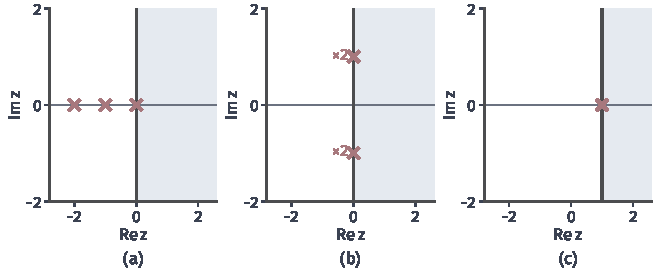
\includegraphics[width=112mm]{figures/06-differential-equations/01-ordinary-differential-equations/matplotlib/lde-laplace-region/figure.pdf}
  \caption{像函数的极点（红叉）与收敛半平面（浅蓝，边界为深灰竖线）。(a)例~\ref{ex:lde-laplace-step}的极点$0,-1,-2$。(b)共振例的二重极点$\pm\mathrm{i}$。(c)$\mathrm{e}^{t}$的极点$1$，收敛范围是$\operatorname{Re}z>1$。}
  \label{fig:lde-laplace-region}
\end{BookInlineFigure}

\paragraph{复极点、重极点与共振}
复极点常用配方处理。对$\ddot{x}+2\dot{x}+5x=0$，$x(0)=1$，$\dot{x}(0)=0$，同样作变换解出$\hat{x}=(z+2)/(z^2+2z+5)$。分母配方为$(z+1)^2+4$，分子写成$(z+1)+1$，于是
\[
 \hat{x}(z)=\frac{z+1}{(z+1)^2+4}+\frac12\cdot\frac{2}{(z+1)^2+4}.
\]
用表中的平移规则和正弦、余弦的变换，得到$x(t)=\mathrm{e}^{-t}(\cos2t+\frac12\sin2t)$，与第~\ref{sec:lde-high-order}节的结果相同。

重极点对应输入与齐次模式的配合。取$\ddot{x}+2\dot{x}+x=\mathrm{e}^{-t}$，零初值。特征根$-1$是二重的，输入又含有同一模式，像函数的极点升到三重：
\[
 \hat{x}(z)=\frac{1}{(z+1)^3}.
\]
由表得$x(t)=\frac12t^2\mathrm{e}^{-t}$。代回检验，
\[
 \dot{x}=\Bigl(t-\frac{t^2}{2}\Bigr)\mathrm{e}^{-t},\qquad
 \ddot{x}=\Bigl(1-2t+\frac{t^2}{2}\Bigr)\mathrm{e}^{-t}.
\]
于是$\ddot{x}+2\dot{x}+x=\mathrm{e}^{-t}$，且$x(0)=\dot{x}(0)=0$。

卷积定理把这一节和常数变易公式联系起来。式~\eqref{eq:lde-forced-oscillator}取$\omega_0=\omega=1$，作变换得
\[
 \hat{x}(z)=\frac{z}{(z^2+1)^2}=\frac{1}{z^2+1}\cdot\frac{z}{z^2+1}.
\]
两个因子分别是$\sin t$和$\cos t$的像，乘积对应卷积$\int_0^t\sin(t-s)\cos s\,\mathrm{d}s$，这正是积分~\eqref{eq:lde-forced-integral}。另一方面，对表中$\mathcal{L}[\sin t](z)=1/(z^2+1)$关于$z$求导，可得$\mathcal{L}[t\sin t](z)=2z/(z^2+1)^2$，于是$x(t)=\tfrac12t\sin t$，与式~\eqref{eq:lde-resonance}相同。二重极点$\pm\mathrm{i}$就是频率上的共振。

\paragraph{分段输入}
延迟规则让分段输入也能一次写出。取$\dot{x}=-x+g$，$x(0)=0$，$g$在$[0,1)$上为$1$，其余时刻为$0$。写$g=\mathbb{I}_{[0,\infty)}-\mathbb{I}_{[1,\infty)}$，得$\hat{g}=(1-\mathrm{e}^{-z})/z$，于是
\[
 \hat{x}(z)=(1-\mathrm{e}^{-z})\Bigl(\frac1z-\frac{1}{z+1}\Bigr).
\]
$1/z-1/(z+1)$对应$1-\mathrm{e}^{-t}$，因子$\mathrm{e}^{-z}$把它延迟$1$，所以
\[
 x(t)=1-\mathrm{e}^{-t}-\bigl(1-\mathrm{e}^{-(t-1)}\bigr)\mathbb{I}_{[1,\infty)}(t).
\]

分段直接解可以验证。在$[0,1)$上是$1-\mathrm{e}^{-t}$；$t\geq1$时方程齐次，从$x(1)=1-\mathrm{e}^{-1}$出发，得$(\mathrm{e}-1)\mathrm{e}^{-t}$。上式在$t\geq1$时化简后也是$(\mathrm{e}-1)\mathrm{e}^{-t}$。$g$在$t=1$跳变，$x$连续但有折角，这是分段输入的绝对连续解。

\paragraph{向量系统与预解矩阵}
对向量系统$\dot{\bm{x}}=\bm{A}\bm{x}+\bm{g}$逐分量作变换，由式~\eqref{eq:lde-laplace-derivative}得到
\[
 (z\bm{I}-\bm{A})\hat{\bm{x}}(z)=\bm{x}_0+\hat{\bm{g}}(z).
\]
矩阵$(z\bm{I}-\bm{A})^{-1}$称为\term{预解矩阵}（resolvent matrix），它把微分方程的传播变成了代数求逆。

\begin{theorem}[矩阵指数的变换]
\label{thm:lde-resolvent}
设$\bm{A}$的特征值实部的最大值为$\gamma$。则对$\operatorname{Re}z>\gamma$，
\begin{equation}
 \mathcal{L}[\mathrm{e}^{t\bm{A}}](z)=\int_0^{\infty}\mathrm{e}^{-zt}\mathrm{e}^{t\bm{A}}\,\mathrm{d}t=(z\bm{I}-\bm{A})^{-1}.
 \label{eq:lde-resolvent}
\end{equation}
于是向量系统的像函数是
\begin{equation}
 \hat{\bm{x}}(z)=(z\bm{I}-\bm{A})^{-1}\bigl(\bm{x}_0+\hat{\bm{g}}(z)\bigr),
 \label{eq:lde-vector-transform}
\end{equation}
它对应时间域的公式~\eqref{eq:lde-duhamel-constant}。
\end{theorem}

\begin{proof}
由定理~\ref{thm:lde-exponential-shape}，$\mathrm{e}^{t\bm{A}}$的元素是$t^j\mathrm{e}^{\lambda t}$的组合，所以对任何$c>\gamma$，存在$C$使下式成立：
\[
 \lVert\mathrm{e}^{t\bm{A}}\rVert_2\leq C\mathrm{e}^{ct}.
\]
取$c$介于$\gamma$与$\operatorname{Re}z$之间，积分绝对收敛。

由定理~\ref{thm:lde-matexp-properties}的(2)，
\[
 \frac{\mathrm{d}}{\mathrm{d}t}\bigl(\mathrm{e}^{-zt}\mathrm{e}^{t\bm{A}}\bigr)=\mathrm{e}^{-zt}\mathrm{e}^{t\bm{A}}(\bm{A}-z\bm{I}).
\]
从$0$积分到$\infty$，左端等于$-\bm{I}$，因为$t\to\infty$时$\mathrm{e}^{-zt}\mathrm{e}^{t\bm{A}}\to\bm{0}$。两边右乘$-(z\bm{I}-\bm{A})^{-1}$；这里$\operatorname{Re}z>\gamma$，$z$不是特征值，矩阵可逆。
\end{proof}

对例~\ref{ex:lde-running-system}的矩阵，
\[
 (z\bm{I}-\bm{A})^{-1}=\frac{1}{(z+1)(z+2)}\begin{bmatrix}z+3&1\\-2&z\end{bmatrix}.
\]
部分分式给出$(1,1)$元$(z+3)/((z+1)(z+2))=2/(z+1)-1/(z+2)$，对应$2\mathrm{e}^{-t}-\mathrm{e}^{-2t}$。$(1,2)$元$1/((z+1)(z+2))=1/(z+1)-1/(z+2)$，对应脉冲响应$w=\mathrm{e}^{-t}-\mathrm{e}^{-2t}$。式~\eqref{eq:lde-resolvent}也说明，因果Green函数$\bm{H}$的变换就是预解矩阵。

\paragraph{方法的边界}
Laplace变换依赖两点：系数是常数，输入是指数阶函数。乘以$t$在变换后变成对$z$求导，所以系数含$t$的方程变成关于$\hat{x}$的微分方程，一般并不比原方程容易。此外，部分分式需要分母的全部根，高阶情形要靠数值计算。这些限制下，第~\ref{sec:lde-time-varying}节的状态转移矩阵和第~\ref{chap:ode-numerical-methods}章的数值方法是必要的。
